\documentclass{article}
\usepackage{imakeidx}
\usepackage{multirow}
\usepackage[a4paper,top=2cm,bottom=2.5cm,left=1.5cm,right=1.5cm,marginparwidth=1.75cm]{geometry}
\usepackage{amsmath}
\usepackage{graphicx}
\usepackage{subfig}
\usepackage{caption}
\usepackage{geometry}
\usepackage{datetime}
\usepackage{wrapfig}
\usepackage[T1]{fontenc}
\usepackage[utf8]{inputenc}
\usepackage[portuguese]{babel}
\usepackage{hyphenat}
\usepackage[export]{adjustbox}
\usepackage[colorlinks=true, allcolors=black]{hyperref}
\usepackage{comment}
\usepackage{blindtext}
\usepackage{graphicx}
\usepackage{float}
\usepackage{tablefootnote}
\usepackage[bottom]{footmisc}
\usepackage[table,xcdraw]{xcolor}
\usepackage{subfig}
\usepackage[utf8]{inputenc}
\usepackage{graphicx}
\usepackage{enumitem}

\begin{document}
\begin{center}
    \begin{minipage}{0.83\linewidth}
        \centering
        
\includegraphics[width=0.4\textwidth]{Images/UM.jpg}\par\vspace{0.5cm}
        {\scshape\textbf{Universidade do Minho}} \par
        {\scshape Licenciatura em Engenharia Informática} \par
        \vspace{3cm}
        {\LARGE Fase 2\\} \par
        {\scshape\LARGE \textbf{Projeto LI3}\\} \par
        \vspace{1.0cm}
        {\LARGE \textbf{Airline Manager}} \par
        \vspace{2cm}
        {\LARGE\textbf {PL6 - Grupo 27}} \par
        \vspace{0.1cm}
        {\LARGE Hugo Abelheira(a95151)\par Luís França(a104259)\par Mariana Rocha(a90817) \par}
        
        \vspace{5cm}
        {\large \today\par}
        
    \end{minipage}
\end{center}
\newpage
\tableofcontents
\listoffigures

\newpage
\section{Introdução}
\paragraph{}A segunda fase deste projeto representa um avanço essencial na implementação do nosso \textit{Query Solver}, concentrando-se em melhorias práticas para a interação do utilizador e na conclusão das funcionalidades pendentes. O foco principal desta fase é a criação de um modo interativo, oferecendo uma interface mais amigável e intuitiva para a execução das \textit{queries} e para manipulação dos dados especificados.
\vspace{-0.3cm}
\paragraph{}Nesta etapa vamos também finalizar as quatro \textit{queries} restantes, proporcionando aos utilizadores um leque mais abrangente de opções para análise de dados. A complexidade adicional traz consigo o desafio contínuo de manter a estrutura modular do projeto, garantindo escalabilidade e eficiência na gestão dos dados específicos fornecidos.
\vspace{-0.3cm}
\paragraph{}Além disso, a introdução de testes funcionais e de desempenho visa validar e aprimorar a viabilidade e eficiência do sistema. Esta abordagem sistemática tem como objetivo consolidar a solidez da solução, proporcionando uma base robusta para o processamento e análise eficaz dos dados específicos do projeto.
\section{Nova Arquitetura e Estruturas}
\subsection{Alterações Iniciais}
\paragraph{}Durante a evolução do projeto, realizamos ajustes estruturais e refinamentos para otimizar a eficiência do sistema. 
\vspace{-0.3cm}
\paragraph{}Simplificamos as estruturas de dados, reduzindo a quantidade de informações armazenadas não apenas para aprimorar o desempenho, mas também para promover uma maior 
escalabilidade. 
\vspace{-0.3cm}
\paragraph{}Além disso, realizamos uma revisão crítica das \textit{hash tables} existentes, eliminando aquelas consideradas desnecessárias. Essa redução não resultou apenas da simplificação, mas, principalmente, de uma análise cuidadosa que revelou estratégias anteriores mais complexas do que o necessário.
\vspace{-0.3cm}
\paragraph{}A decisão de eliminar o módulo \textit{statistics} foi acompanhada pela redistribuição estratégica do seu conteúdo, integrando-o em áreas que se alinham melhor com a lógica de negócio e a modularidade do sistema. 
\vspace{-0.3cm}
\paragraph{}Simultaneamente, introduzimos novas \textit{hash tables} eficientes, projetadas para lidar especificamente com desafios de \textit{queries} particulares. 
\vspace{-0.3cm}
\paragraph{}Essas mudanças não só simplificaram a estrutura global e fortaleceram a coesão do código, mas também contribuíram para um sistema mais ágil e preparado para futuras expansões, com uma gestão de \textit{hash tables} mais eficiente.
\subsection{Arquitetura}
\paragraph{}Ao conceber a arquitetura deste projeto, mantivemos uma abordagem modular que se baseou na estrutura previamente estabelecida na fase anterior, com a incorporação essencial do modo interativo nesta segunda fase. O sistema permanece dividido em três componentes principais: \textbf{Processamento de Entrada}, \textbf{Lógica de Negócios} e \textbf{Geração de Resultados}. Essa organização modular permite uma implementação robusta e escalável, onde cada módulo desempenha funções específicas, contribuindo para a coesão global do sistema.
\vspace{-0.3cm}
\paragraph{}No âmbito da \textbf{modularidade}, cada componente opera independentemente, facilitando a manutenção, a expansão e a compreensão individual das suas funcionalidades. A estrutura modular oferece flexibilidade, permitindo ajustes e adições sem afetar outras partes do sistema. Esta abordagem foi crucial para a incorporação do modo interativo, uma vez que adicionamos funcionalidades sem comprometer a estabilidade global do programa.
\vspace{-0.3cm}
\paragraph{}Quanto ao \textbf{encapsulamento}, cada módulo encapsula as suas operações internas, expondo apenas as interfaces necessárias para interações externas. Essa prática não apenas promove a segurança e a integridade dos dados, mas também simplifica a compreensão e o uso do sistema. A estratégia de encapsulamento permaneceu consistente ao longo do trabalho, garantindo uma implementação coesa e de fácil manutenção.
\vspace{-0.3cm}
\paragraph{}A Figura 1 apresenta um diagrama simplificado que ilustra as principais classes e suas interações no sistema. Este diagrama proporciona uma visão visual clara da estrutura do projeto.
\begin{figure}[H]
\begin{center}
	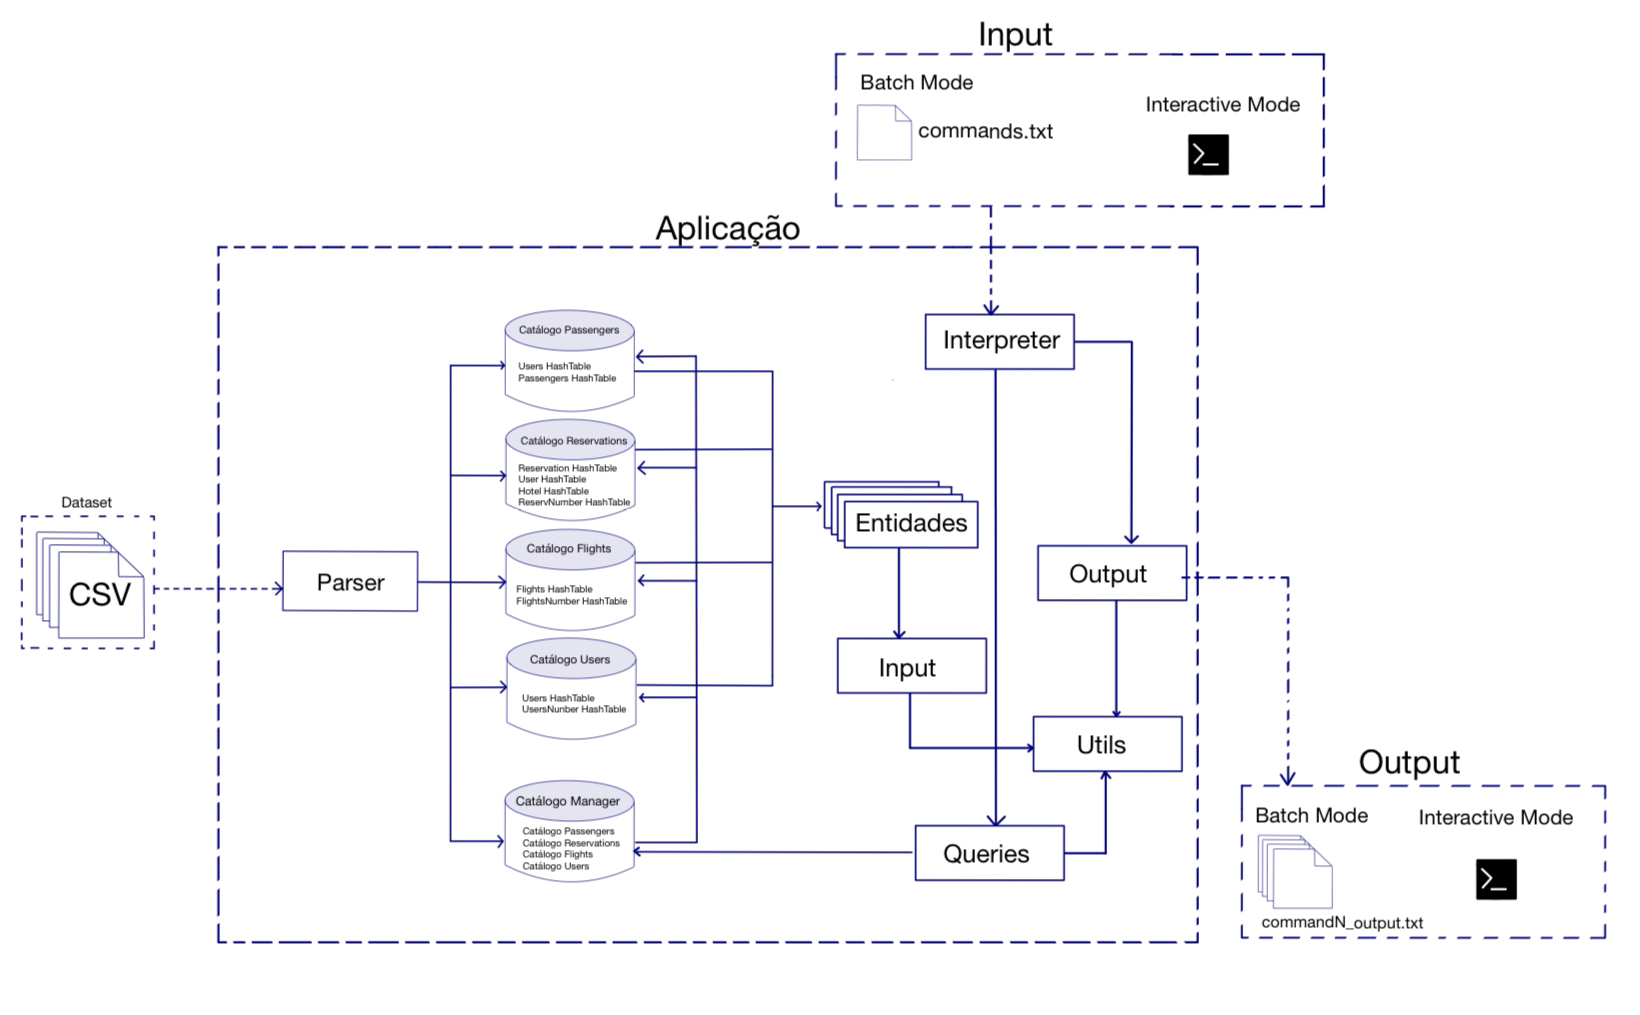
\includegraphics[width=15cm]{Images/arquitetura.jpeg} 
        \caption{Representação da Arquitetura do Projeto}
\end{center}
\end{figure}


\subsection{Queries}
\paragraph{}\textbf{Query 7:} "Listar o \textit{top N} aeroportos com a maior mediana de atrasos. Atrasos num aeroporto são calculados a partir da diferença entre a data estimada e a data real de partida, para voos com origem nesse aeroporto. O valor do atraso deverá ser apresentado em segundos. Caso dois aeroportos tenham a mesma mediana, o nome do aeroporto deverá ser usado como critério de desempate (de forma crescente)."

A \textit{query} 7 tem como objetivo listar o \textit{top N} aeroportos com a maior mediana de atrasos. Utilizando uma estrutura de dados denominada \textit{AirportInfo2}, o código itera sobre os voos armazenados no catálogo, calculando os atrasos com base na diferença entre as datas estimada e real de partida. Esses atrasos são acumulados num \textit{array} dinâmico, associados a cada aeroporto. A mediana dos atrasos é então calculada para cada aeroporto, e o array de \textit{AirportInfo2} é ordenada utilizando a função \textit{qsort}. A função retorna os resultados formatados, limitados ao \textit{top N} aeroportos com as maiores medianas de atrasos, após a devida libertação da memória alocada para evitar quaisquer \textit{memory leaks}.

\paragraph{}\textbf{Query 8:} "Apresentar a receita total de um hotel entre duas datas (inclusive), a partir do seu identificador. As receitas de um hotel devem considerar apenas o preço por noite (\textit{price\_per\_night}) de todas as reservas com noites entre as duas datas. E.g., caso um hotel tenha apenas uma reserva de 100Eur/noite de 2023/10/01 a 2023/10/10, e quisermos saber as receitas entre 2023/10/01 a 2023/10/02, deverá ser retornado 200Eur (duas noites). Por outro lado, caso a reserva seja entre 2023/10/01 a 2023/10/02,
deverá ser retornado 100Eur (uma noite)."

A \textit{query} 8 é destinada a apresentar a receita total de um hotel entre duas datas, considerando o preço por noite das reservas. A função utiliza um identificador de hotel e intervalo de datas como argumentos. A lógica consiste em iterar sobre as reservas associadas ao hotel, verificando se as datas da reserva estão contidas no intervalo especificado. Caso haja sobreposição, a função calcula o número de noites dentro desse intervalo e soma o preço por noite multiplicado pelo número de noites à receita total do hotel. O resultado final é retornado como uma \textit{string} representando o valor total da receita.

\paragraph{}\textbf{Query 9:} "Listar todos os utilizadores cujo nome começa com o prefixo passado por argumento, ordenados
por nome (de forma crescente). Caso dois utilizadores tenham o mesmo nome, deverá ser usado o seu identificador como critério de desempate (de forma crescente). Utilizadores inativos não deverão ser considerados pela pesquisa."

A \textit{query} 9 foi projetada para listar todos os utilizadores cujo nome começa com o prefixo passado por argumento, ordenados por nome de forma crescente. Em caso de nomes iguais, o identificador é utilizado como critério de desempate também de forma crescente. A função exclui utilizadores inativos da pesquisa, percorrendo a tabela de utilizadores, identificando aqueles que atendem aos critérios e armazenando as informações em uma estrutura dinâmica chamada \textit{User\_list}. Posteriormente, os resultados são ordenados usando a função \textit{qsort} e formatados num \textit{array} de \textit{strings} representando o número total de utilizadores encontrados, juntamente com detalhes sobre cada utilizador, como identificador e nome. A memória, como sempre, é gerida para evitar \textit{leaks}.

\paragraph{}\textbf{Query 10:} "Apresentar várias métricas gerais da aplicação. As métricas consideradas são: número de novos utilizadores registados (de acordo com o campo \textit{account\_creation}); número de voos (de acordo com o campo \textit{schedule\_departure\_date}); número de passageiros; número de passageiros únicos; e 12 número de reservas (de acordo com o campo begin\_date). Caso a \textit{query} seja executada sem argumentos, apresentar os dados agregados por ano, para todos os anos que a aplicação tem registo. Caso a \textit{query} seja executada com um argumento, \textit{year}, apresentar os dados desse ano agregados por mês. Finalmente, caso a \textit{query} seja executada com dois argumentos, \textit{year} e \textit{month}, apresentar os dados desse ano e mês agregados por dia. O output deverá ser ordenado de forma crescente consoante o ano/mês/dia.


A \textit{query} 10, destinada a apresentar diversas métricas gerais da aplicação, incluindo o número de novos utilizadores registados, voos, passageiros, passageiros únicos e reservas. A apresentação dessas métricas varia conforme os argumentos fornecidos à \textit{query}: sem argumentos, os dados são agregados por ano para todos os anos registados; com um argumento (\textit{year}), os dados desse ano são apresentados agregados por mês; com dois argumentos (\textit{year} e \textit{month}), os dados desse ano e mês são apresentados agregados por dia. A função utiliza estruturas de dados e funções auxiliares para processar as informações dos catálogos e gera um \textit{array} de \textit{strings} representando as métricas agregadas, ordenadas de forma crescente. A gestão de memória é realizada de forma apropriada para prevenir possíveis \textit{memory leaks}.

\section{Modo Interativo}
\paragraph{}Nesta secção, abordaremos detalhadamente o modo interativo do nosso projeto, implementado utilizando a biblioteca \textit{NCurses}. Desenvolvemos uma série de menus intuitivos que oferecem aos utilizadores uma experiência mais amigável e acessível com o nosso \textit{Query Solver}. A inclusão de uma aba de instruções fornece informações relevantes, permitindo que os usuários explorem as funcionalidades do sistema de forma eficiente e percetível. Adicionalmente, incorporamos um menu de configurações, visando melhorar a qualidade de vida do usuário, proporcionando ajustes personalizáveis para uma experiência mais adaptada e eficaz. Essas inovações não apenas facilitam a interação com o \textit{Query Solver}, mas também reforçam o nosso compromisso com uma interface mais intuitiva e centrada no utilizador.
\subsection{Requisitos}
\subsubsection{Não Funcionais}
\begin{itemize}
\item O caminho padrão sugerido deve ser conveniente para o usuário e, quando possível, relativo à pasta de execução do programa.
\item O \textit{layout} dos resultados deve ser claramente definido, proporcionando uma apresentação organizada e legível das informações.
\item A personalização do formato de output deve ser eficiente e intuitiva para melhorar a experiência do utilizador.
\item O sistema de paginação deve ser eficiente para lidar com grandes conjuntos de dados, garantindo uma resposta rápida e uma navegação suave.
\item O sistema de navegação por setas deve ser intuitivo, proporcionando uma experiência de usuário agradável e sem complicações.
\item Quando ocorrerem erros por parte do utilizador, uma caixa de texto colorida deve ser exibida para destacar e explicar claramente o argumento inserido incorretamente.
\item A aba de instruções deve ser apresentada de forma clara e intuitiva, garantindo que o utilizador possa entender facilmente como interagir com o programa e fornecendo exemplos práticos.
\item A aba de \textit{settings} deve ser de fácil acesso e compreensão, proporcionando uma configuração conveniente e rápida antes do início do programa.
\item Mesmo seguindo um formato específico, o design do input deve ser intuitivo, facilitando a inserção correta de informações por parte do utilizador e minimizando possíveis erros devido a ambiguidades.
\end{itemize}
\subsubsection{Funcionais}
\begin{itemize}
    \item O programa deve ser capaz de iniciar sem a necessidade de argumentos e, quando necessário, sugerir um caminho padrão relativo à pasta de execução do programa.
    \item O modo interativo deve fornecer instruções claras para cada \textit{query} disponível, orientando o utilizador sobre como formatar e inserir as consultas.
    \item O sistema deve incluir um módulo de paginação para lidar com resultados extensos, permitindo ao usuário navegar pelos dados de maneira eficiente.
    \item O programa deve adotar um formato de input padronizado para cada \textit{query}, conforme detalhado nas instruções, proporcionando consistência e previsibilidade na interação do usuário com o sistema.
    \item O programa deve permitir ao utilizador a escolha do formato de \textit{output}, incluindo as opções de visualização num ficheiro \textit{txt}, visualização por número de páginas ou por número de \textit{outputs} ou um por um.
    \item O sistema deve ser capaz de identificar e lidar graciosamente com erros comuns do usuário, como inserção inadequada de texto em \textit{queries} de \textit{top N} ou especificação de uma pasta inválida para o \textit{dataset}.
    \item Deve existir um sistema de navegação por setas para facilitar a movimentação do usuário dentro do programa, especialmente ao explorar os resultados paginados.
    \item O modo interativo deve incluir uma aba de instruções que forneça informações detalhadas sobre o funcionamento do programa, exemplos do \textit{input} para diferentes \textit{queries} e exemplos de \textit{outputs} esperados.
\end{itemize}
\subsection{Desenvolvimento}
\paragraph{}Iniciamos o desenvolvimento do modo interativo implementando uma página inicial que apresenta as principais opções do programa, nomeadamente o \textit{Airline Query Solver}, que encapsula toda a lógica de negócio, uma aba de instruções detalhada e a opção \textit{Exit} para encerrar o programa. A aba de instruções foi estruturada em três páginas distintas: a primeira fornece uma introdução ao sistema e o seu propósito, a segunda explica em detalhes o funcionamento do programa, e a terceira contém informações específicas de cada \textit{query}, incluindo um resumo, exemplos de \textit{input} e exemplos de \textit{output} corretos.
\vspace{-0.3cm}
\paragraph{}Ao entrar no \textit{Airline Query Solver}, o utilizador é recebido com uma aba de \textit{settings} que permite a personalização de aspetos como a \textit{path} do \textit{dataset} e os formatos de output, conforme especificado nos requisitos. Após a configuração, os catálogos são preenchidos com a informação da \textit{path} fornecida, e o sistema avança para o \textit{Query Solver}. Caso ocorram problemas, o programa está preparado para apresentar mensagens e códigos de erro, garantindo uma experiência informativa.
\vspace{-0.3cm}
\paragraph{}No \textit{Query Solver}, o utilizador tem a oportunidade de especificar a \textit{query} desejada e os respetivos argumentos, personalizados para cada \textit{query} individual. Destaca-se a atenção especial dada aos menus e à qualidade de vida do utilizador, com a inclusão de notas explicativas que o acompanham ao longo do programa. Por exemplo, se o formato da data inserida for inválido, será exibida de mensagem de erro no menu flutuante em questão, evitando que o utilizador perca tempo inserindo os outros argumentos.
\vspace{-0.3cm}
\paragraph{}O menu final, denominado \textit{Query Result}, permite a visualização dos \textit{outputs} de acordo com o formato escolhido nas \textit{settings}. As opções incluem \textit{One by One}, \textit{Txt Format} para exportar para ficheiros \textit{txt}, escolher o número de páginas ou definir o número de \textit{outputs} por página. Cada uma destas opções será detalhadamente explorada a seguir. 
\begin{itemize}
    \item Txt Format: Ao escolher esta opção, o utilizador solicita a geração de um ficheiro \textit{txt} contendo o \textit{output} da \textit{query} selecionada. Esta abordagem permite uma fácil exportação e partilha dos resultados, tornando a gestão da informação obtida bastante prática.
    \item One by One: Optando por este formato, cada \textit{output} é apresentado individualmente. O utilizador pressiona a tecla "c" (de \textit{continue}) para avançar para o próximo resultado. Quando a janela atinge a capacidade máxima, é criada uma nova página, mantendo a apresentação dos \textit{outputs} de forma sequencial.
    \item Number of Pages: Nesta opção, o utilizador especifica o número desejado de páginas para visualização dos \textit{outputs}. Os resultados são distribuídos de maneira proporcional, sendo importante notar que, caso o número de total de outputs seja superior ao limite da página, será necessário fazer \textit{scroll down} para aceder aos restantes resultados dessa página.
    \item Number of Outputs per Page: Ao indicar a quantidade de \textit{outputs} desejada por página, o sistema calcula automaticamente o número total de páginas necessárias para apresentar todos os resultados. Importante salientar que, se o utilizador solicitar mais \textit{outputs} por página do que a janela consegue mostrar, será necessário utilizar a opção de \textit{scroll down} para visualizar os resultados adicionais na mesma página.
\end{itemize}

\subsection{Interface Final}
\paragraph{}A apresentação visual do nosso sistema final é exemplificada pelas figuras abaixo que revelam a interface gráfica dos menus desenvolvidos. Estes \textit{snapshots} fornecem uma visão prática dos diferentes menus, demonstrando a organização, opções e a interatividade intuitiva que os utilizadores podem esperar ao utilizar o nosso sistema. Cada imagem destaca um aspeto específico da interface final, proporcionando uma representação sucinta da experiência visual global.
\begin{figure}[H]
\begin{center}
	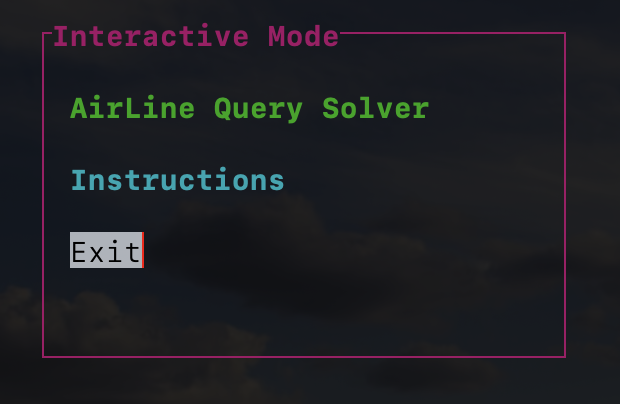
\includegraphics[width=6cm]{Images/home.png}
        \quad\quad\quad\quad\quad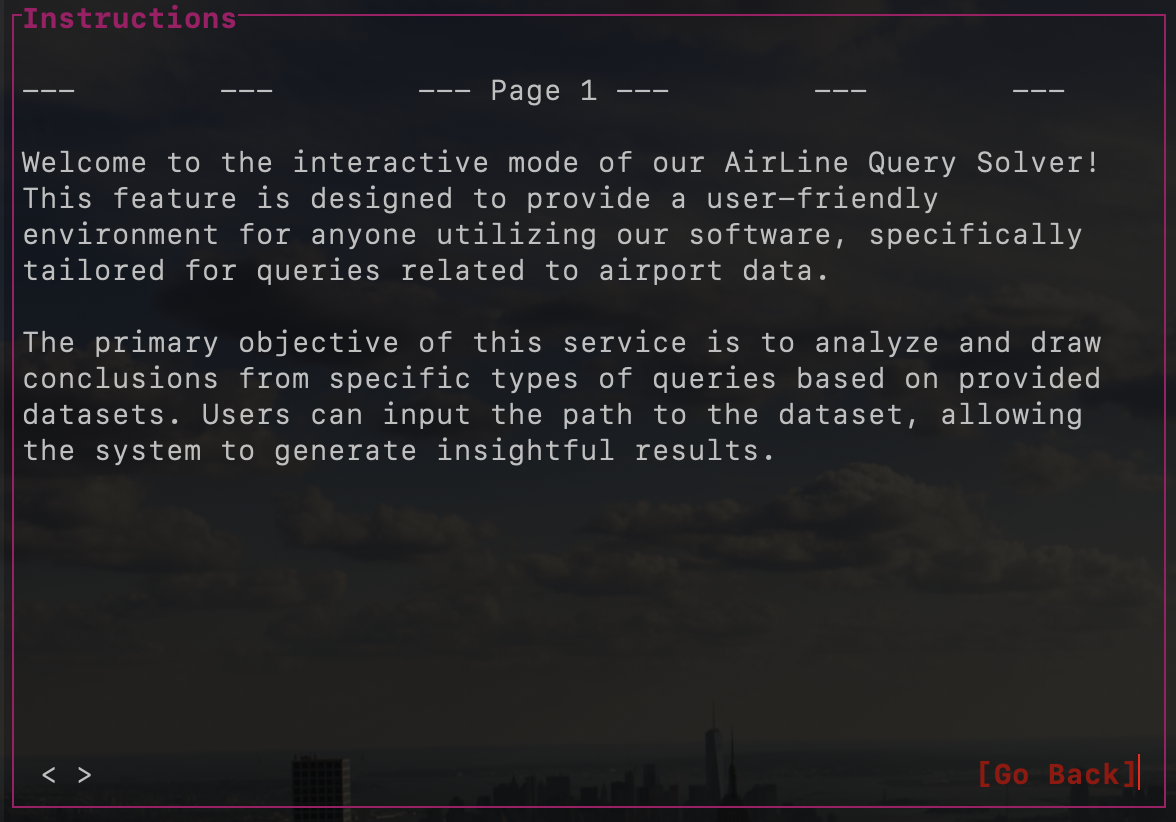
\includegraphics[width=5.5cm]{Images/instru.png} 
        \caption{Home e Instructions Page}
\end{center}
\end{figure}
\begin{figure}[H]
\begin{center}
        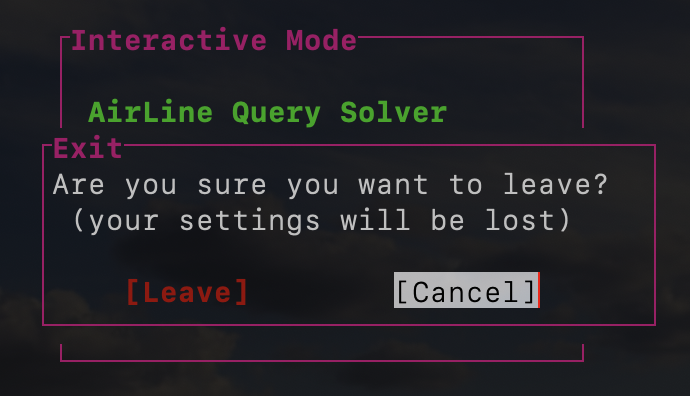
\includegraphics[width=6.5cm]{Images/exit.png} 
        \quad\quad\quad\quad\quad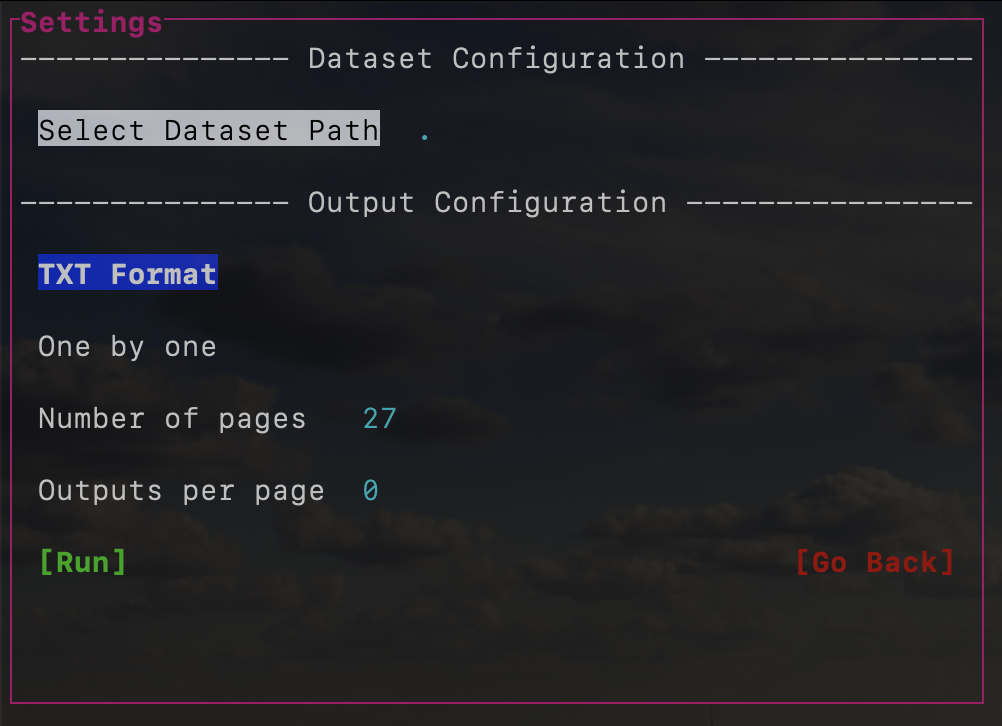
\includegraphics[width=5.5cm]{Images/settings.png} 
        \caption{Exit Option e Settings Page} 
\end{center}
\end{figure}
\begin{figure}[H]
\begin{center}
        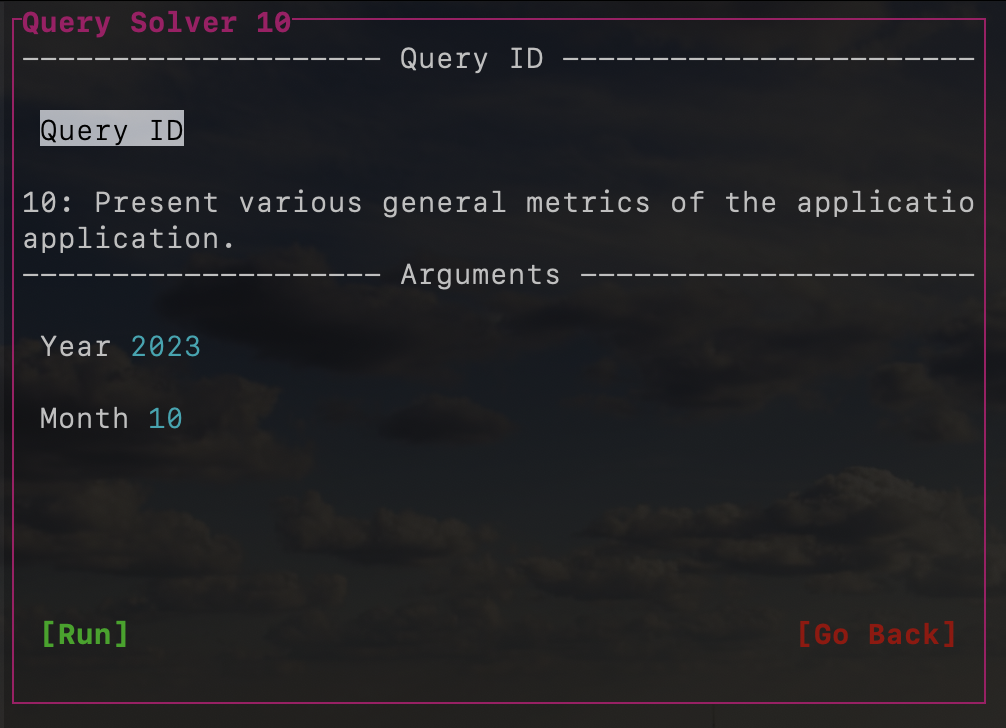
\includegraphics[width=5.5cm]{Images/solver.png} 
        \quad\quad\quad\quad\quad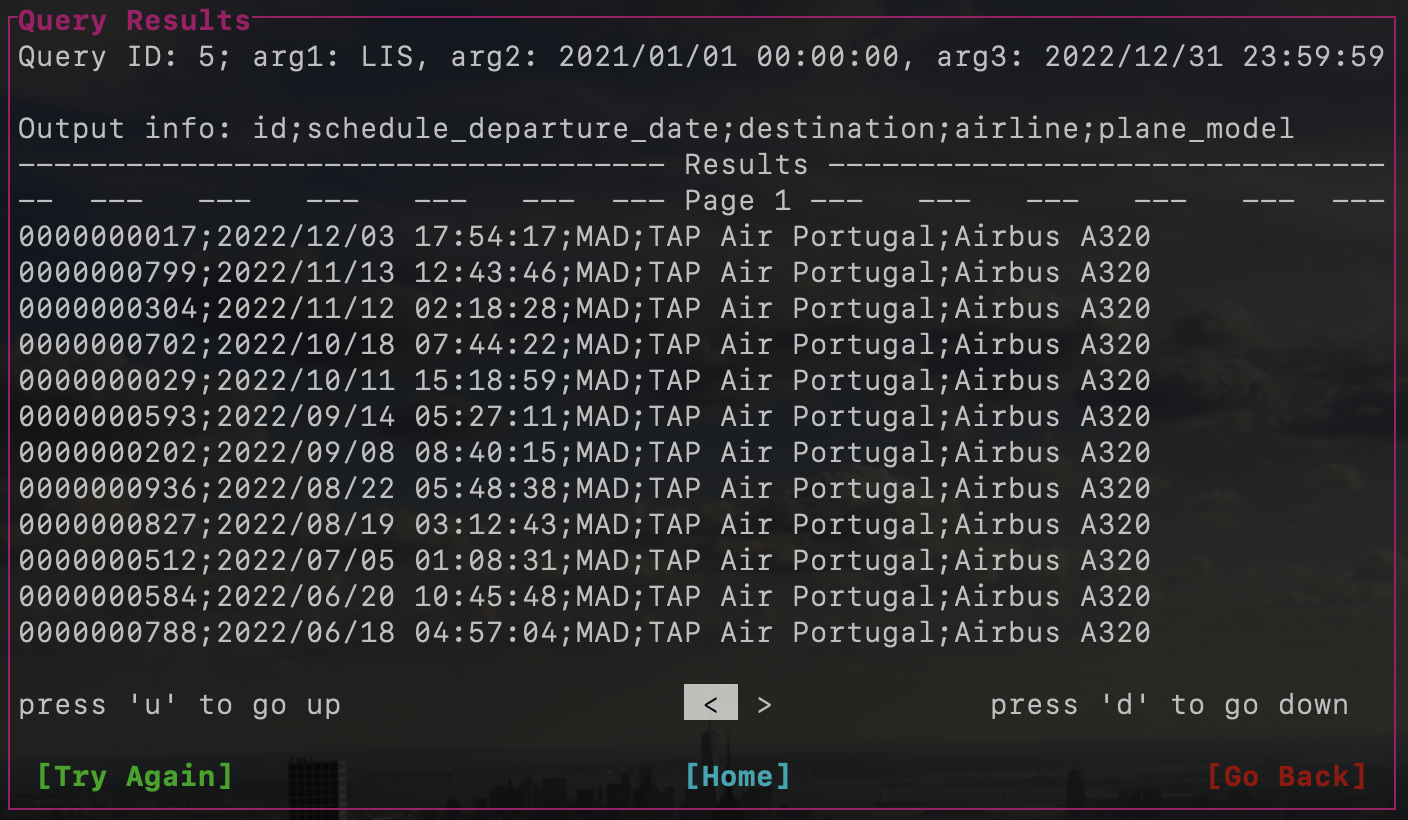
\includegraphics[width=6.5cm]{Images/result.png}
        \caption{Query Solver e Result Pages}
\end{center}
\end{figure}
\section{Testes} 
\paragraph{}Os testes funcionais foram essenciais para verificar a correta implementação das funcionalidades do sistema, validando a lógica e a precisão das respostas. Em paralelo, os testes de desempenho abordaram métricas críticas, como tempo de execução das \textit{queries} e uso eficiente da memória, proporcionando uma análise abrangente do desempenho do sistema em diferentes cenários.
\vspace{-0.3cm}
\paragraph{}Os \textbf{testes funcionais} foram concebidos seguindo os mesmos princípios de modularidade e encapsulamento. Cada teste avalia individualmente a funcionalidade específica de uma \textit{query}, isolando-a de outras partes do sistema. Essa abordagem não apenas facilita a identificação e correção de problemas, mas também contribui para a confiabilidade geral do sistema, garantindo que cada módulo funcione conforme o esperado, mesmo em cenários de interação complexa.
\vspace{-0.3cm}
\paragraph{}Para os testes funcionais, adotamos uma abordagem específica, utilizando a técnica que os professores sugeriram para verificar a correta execução das \textit{queries}. Desenvolvemos uma variedade de testes para cada \textit{query}, variando os tipos de argumentos (válidos e inválidos) para garantir uma cobertura abrangente. Cada teste incluiu a medição do tempo de execução, proporcionando uma compreensão sobre a eficiência de cada \textit{query} em diferentes condições.
\vspace{-0.3cm}
\paragraph{}No âmbito dos \textbf{testes de desempenho}, também seguimos as orientações fornecidas pelos docentes. Implementamos um "programa-testes" que recebe o caminho para o \textit{dataset}, o ficheiro txt de comandos e a pasta com os resultados esperados. Este programa compara os resultados obtidos com os esperados, indicando se o teste foi bem-sucedido ou apontando a linha da primeira incongruência encontrada. Além disso, registamos o tempo de execução de cada \textit{query} e o tempo geral de execução, bem como a quantidade de memória utilizada pelo programa.
\vspace{-0.3cm}
\paragraph{}Os valores dos testes funcionais podem ser consultados no arquivo \texttt{analysis.txt}, enquanto a análise de desempenho está disponível no arquivo \texttt{analysisTest.txt}.


\section{Análise de Desempenho}
\paragraph{}A análise de desempenho desempenha um papel crucial na avaliação da eficácia e eficiência do sistema desenvolvido. Nesta secção são explorados os resultados dos testes realizados em diferentes máquinas, proporcionando uma visão aprofundada do comportamento do sistema em cenários diversos.
\vspace{-0.3cm}
\paragraph{}Mostraremos dados quantitativos sobre o tempo de execução de cada \textit{query}, o tempo geral de execução do sistema e a quantidade de memória utilizada. Essas métricas fornecerão perceções significativas sobre a eficiência operacional do sistema, permitindo-nos entender melhor como ele responde a diferentes demandas de processamento.
\vspace{-0.3cm}
\paragraph{}Este capítulo destaca a importância de compreender não apenas a funcionalidade individual das \textit{queries}, mas também o impacto coletivo delas no desempenho global do sistema.
\vspace{-0.3cm}
\paragraph{}Apresentamos a tabela seguinte que contem as médias dos tempos de execução obtidos ao realizar o programa de testes em cada máquina, 10 iterações de 100 \textit{queries}. Este conjunto diversificado de execuções permite uma visão abrangente do desempenho do sistema sob várias condições. Além das médias dos tempos de execução, fornecemos informações específicas sobre cada computador utilizado, destacando particularidades relevantes para a análise dos resultados.

\begin{table}[h]
\begin{center}
\begin{tabular}{|c|c|c|c|} 
\rowcolor{lightgray}
\hline
  & Máquina 1 & Máquina 2 & Máquina 3 \\ % inserts table
%heading
\hline
\cellcolor{lightgray} Modelo & Acer SF315-41-R34L & MackBook Pro 2020 & HP 15s-fq1028np\\
\hline % insere única linha horizontal
\cellcolor{lightgray} CPU & amd ryzen 5 & i5 & i7\\
\hline
\cellcolor{lightgray}RAM & 8Gb & 16Gb & 12Gb\\
\hline
\cellcolor{lightgray}Sistema Operacional & Zorin OS & MacOS & Ubuntu \\
\hline
\cellcolor{lightgray}Compilador & gcc 12.2.1 & Apple clang 15.0.0 & gcc 11.4.0 \\
\hline
\cellcolor{lightgray}Memória máxima do programa & 33Mb & \textit{Error} & 33Mb \\
\hline
\cellcolor{lightgray}Tempo de execução & 0.32s & 0.37s & 0.49s \\
\hline
\end{tabular}
\caption{Tabela Informativa}
\label{table:nonlin}
\end{center}
\end{table}
\vspace{-0.3cm}
\paragraph{}Embora os computadores com hardware mais avançado demonstrem tempos de execução superiores em relação ao computador com desempenho inferior, é importante notar que as diferenças observadas não são significativamente pronunciadas. A marginal discrepância nos tempos de execução sugere que, apesar das variações no hardware, o sistema mantém uma consistência notável em sua capacidade de resposta. Essa relativa uniformidade indica uma eficiência robusta do sistema, capaz de fornecer resultados satisfatórios mesmo em ambientes com configurações de hardware distintas. Essa constância no desempenho contribui para a versatilidade do sistema, adaptando-se efetivamente a diferentes contextos de utilização.
\vspace{-0.3cm}
\begin{figure}[H]
\begin{center}
        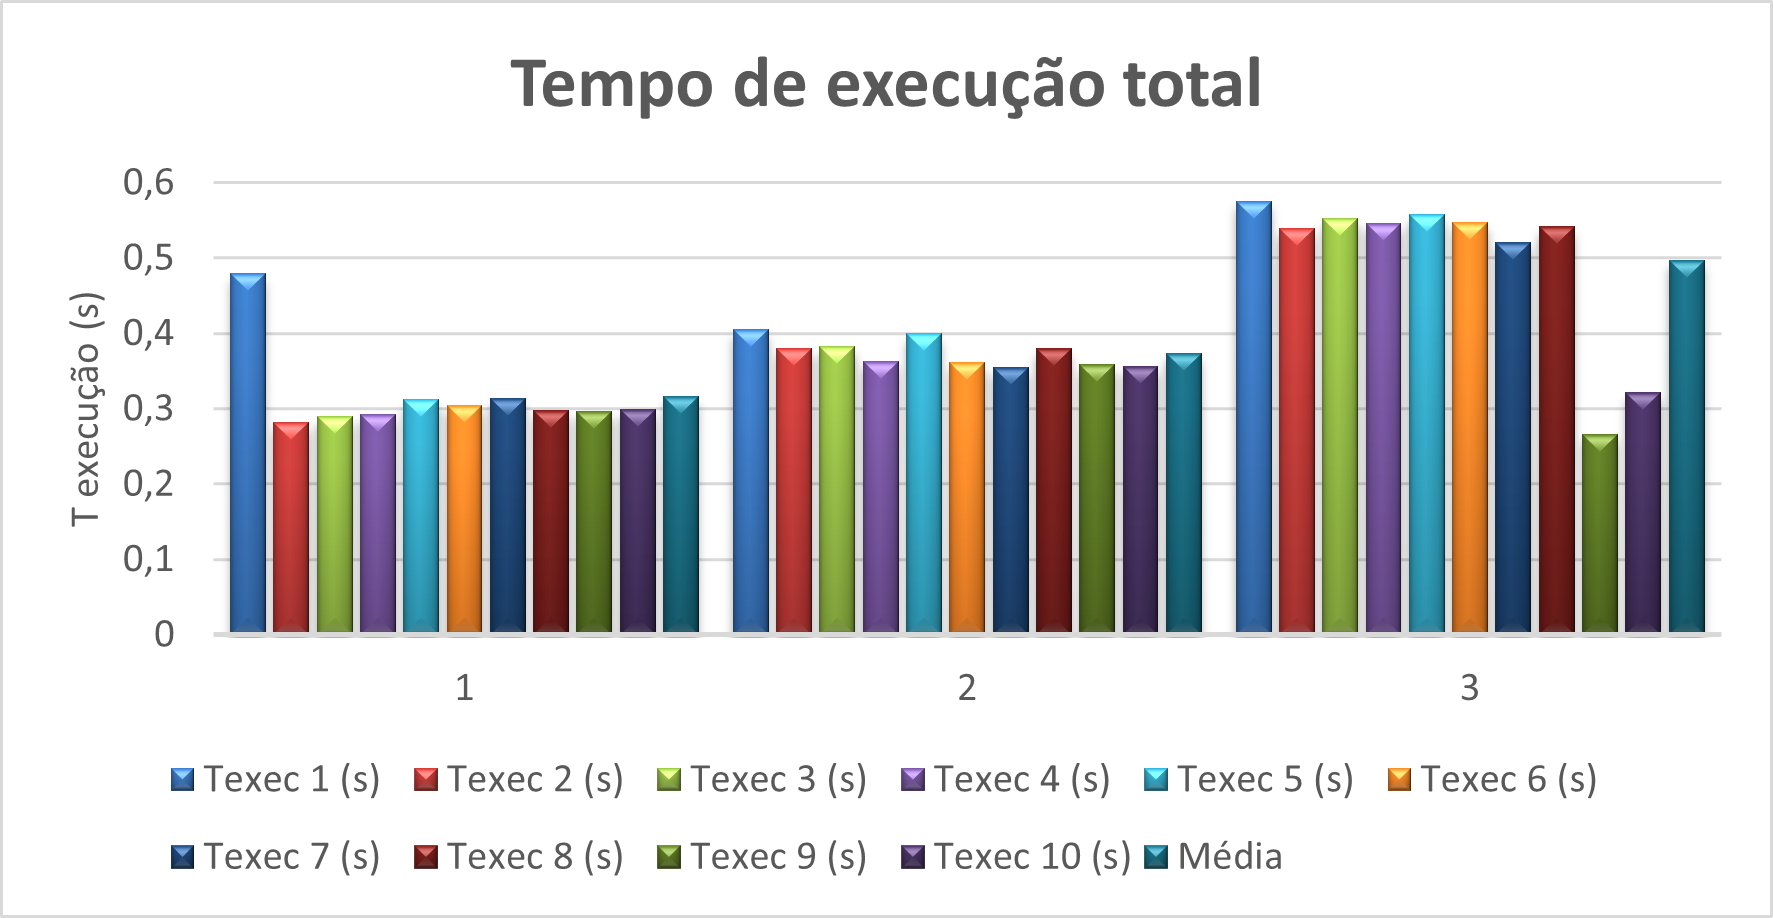
\includegraphics[width=8.5cm]{Images/TempoExecucao.png} 
        \quad\quad\quad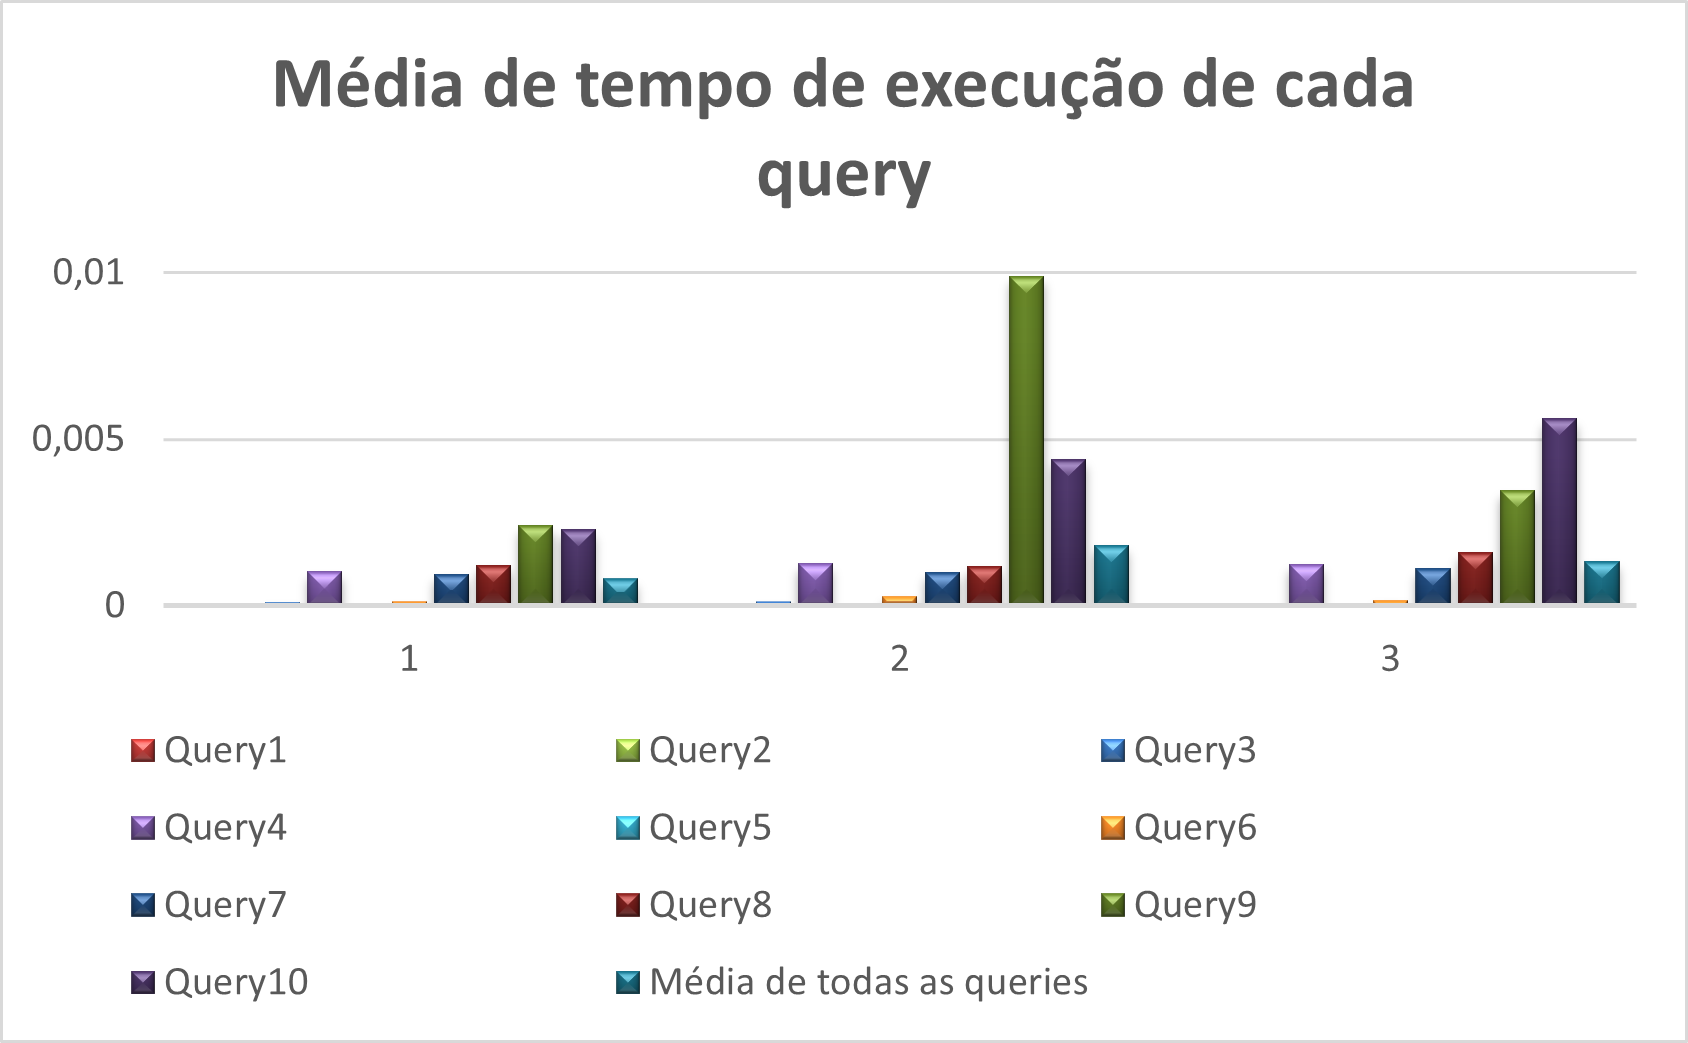
\includegraphics[width=7cm]{Images/Query.png} 
        \caption{Tempo de execução por máquina e média de tempo de execução de cada query} 
\end{center}
\end{figure}
\paragraph{}Os valores baixos de execução de \textit{queries} refletem a eficiência das escolhas de estruturas de dados adotadas no projeto. A utilização extensiva de \textit{hashtables} contribui significativamente para tempos de acesso rápidos aos dados. Além disso, a implementação de \textit{hashtables} específicas para determinadas \textit{queries} otimiza ainda mais o desempenho, oferecendo um acesso mais eficiente aos dados relevantes.
\vspace{-0.3cm}
\paragraph{}A decisão de empregar a função \textit{qsort} para a ordenação de dados nas \textit{queries} necessárias também se alinha com a busca pela eficiência. A complexidade assintótica de O(N*log N) desta função torna-a numa escolha apropriada para ordenar conjuntos de dados, garantindo um processamento rápido e escalável, essencial para operações que envolvem a organização eficiente de informações em diferentes contextos.
\vspace{-0.3cm}
\paragraph{}Estas escolhas fundamentadas nas características das estruturas de dados e nas complexidades algoritmias contribuem de forma significativa para o desempenho global do sistema, assegurando uma resposta ágil e eficaz na execução das \textit{queries} propostas.

\subsection{Valgrind}
\paragraph{}Começamos por resolver os 100 \textit{bytes} de \textit{memory leaks} do sistema. A partir desse ponto, mantivemos a libertação de memória total na evolução da segunda fase, resultando na ausência de \textit{leaks} tanto no programa principal quanto no programa de teste, conforme pode ser verificado nas imagens em anexo. Este progresso não apenas resolveu desafios específicos, mas também reflete o nosso compromisso contínuo com a eficiência operacional.

\begin{figure}[H]
\begin{center}
	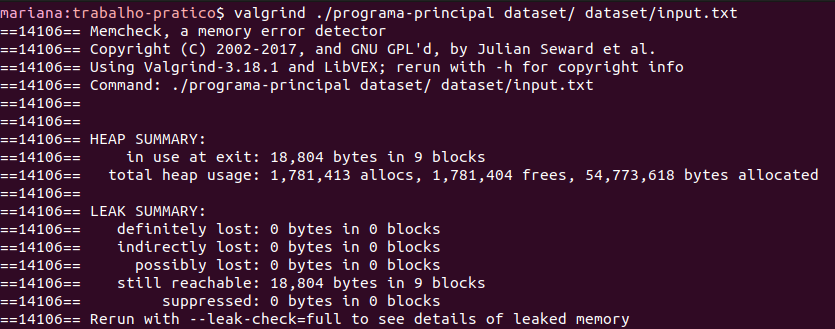
\includegraphics[width=7.5cm]{Images/leaksPrincipal.png}
        \quad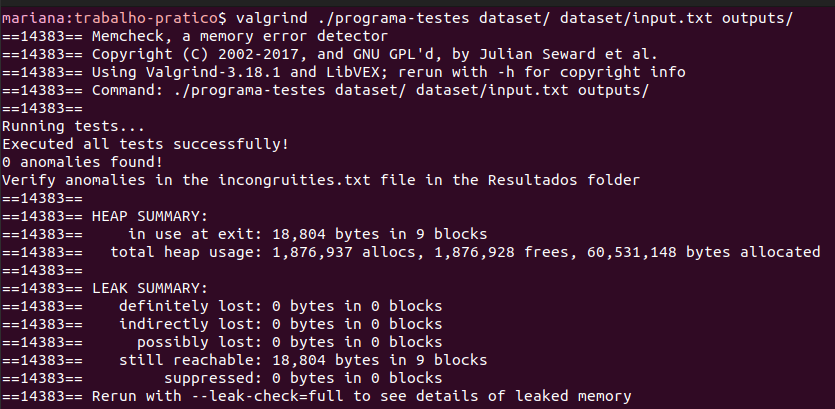
\includegraphics[width=6cm]{Images/leaksTest.png} 
        \caption{Quantidade de \textit{memory leaks} do programa-principal e do programa-testes}
\end{center}
\end{figure}

\paragraph{}Ao longo do desenvolvimento, a atenção proativa à resolução de \textit{leaks} iniciais contribuiu para melhorar a estabilidade do sistema e estabelecer uma base sólida para a gestão eficiente de recursos.
\vspace{-0.3cm}
\paragraph{}Em resumo, ao superar desafios iniciais e manter uma abordagem diligente na gestão de memória, conseguimos criar um sistema mais robusto e eficiente, agora livre de qualquer tipo de \textit{memory leak}.

\section{Dificuldades Sentidas}
\paragraph{}O desenvolvimento do modo interativo e a preparação para avaliação do sistema não estiveram isentos de desafios. À medida que exploramos a implementação detalhada do modo interativo, desde a criação da página inicial até o sistema de outputs flexíveis, identificamos obstáculos que exigiram soluções engenhosas. Simultaneamente, a etapa de preparação para a avaliação do sistema envolveu desafios específicos relacionados aos testes funcionais e de desempenho, incluindo monitoramento de memória e otimização de tempo de execução. Este capítulo discute esses desafios, apresentando uma perspetiva abrangente sobre como foram abordados, proporcionando uma base para as conclusões finais.
\subsection{Modo Interativo}
\paragraph{}O desenvolvimento do modo interativo envolveu superar desafios significativos. A aprendizagem da biblioteca \textit{NCurses}, a gestão eficaz de memória, a implementação de encapsulamento modular e a lógica de negócios associada à manipulação de catálogos e apresentação de \textit{outputs} requereram esforços específicos para garantir um sistema robusto e eficiente. Estas adversidades contribuíram para o aprimoramento das habilidades de desenvolvimento, resultando numa solução que atende aos padrões mais elevados de qualidade e usabilidade.
\subsection{Avaliação do Sistema}
\paragraph{}A fase de testes funcionais e de desempenho, embora mais acessível por causa do código fornecido pelos professores, não esteve isenta de desafios. Enfrentamos uma complexidade adicional relacionada ao sistema operativo, especialmente no ambiente \textit{MacOS}. Um problema peculiar surgiu ao calcular a utilização de memória, onde, mesmo com um uso real de aproximadamente 32 MB, o \textit{MacOS} indicava erroneamente um consumo de 25 GB, uma discrepância que, até o momento, permanece sem uma solução clara. Este obstáculo destacou a importância de considerar as nuances dos diferentes sistemas operativos para garantir uma avaliação precisa do desempenho do sistema.
\section{Conclusão}
\paragraph{}Ao longo deste projeto, embarcamos numa jornada para criar um sistema robusto e eficiente de gestão de dados. Desde a fase inicial, onde delineamos a arquitetura e realizamos adaptações estruturais, até à implementação do modo interativo com foco em otimizações de \textit{queries} e experiência do usuário, buscamos constantemente a excelência. A eliminação de módulos desnecessários e a reestruturação eficiente das \textit{hash tables} refletem a nossa dedicação à lógica de negócios e a conceitos teóricos como a modularidade e o encapsulamento.
\vspace{-0.3cm}
\paragraph{}A introdução de um modo interativo, desenvolvido utilizando a biblioteca \textit{NCurses}, apresenta uma interface intuitiva e amigável para interação com o sistema. Os menus, abas de instruções e configurações proporcionam uma experiência coesa e simplificada, refletindo a atenção cuidadosa dada à qualidade de vida do utilizador.
\vspace{-0.3cm}
\paragraph{}As dificuldades enfrentadas durante o desenvolvimento, especialmente na criação do modo interativo e na preparação para a avaliação do sistema, destacaram a nossa busca incessante pela perfeição. A abordagem sistemática nos testes funcionais e de desempenho permitiu-nos garantir não apenas a funcionalidade correta, mas também a eficiência operacional.
\vspace{-0.3cm}
\paragraph{}Olhando para o futuro, este projeto não é apenas um sistema bem sucedido, mas também um exemplo de escalabilidade e adaptabilidade. As alterações estratégicas implementadas ao longo do desenvolvimento e o cuidado constante na gestão de recursos estabelecem uma base sólida para futuras expansões e melhorias.
\end{document}
